\documentclass[10 pt]{article}
\usepackage{multicol}
\usepackage[ portrait, margin = 0.7 in]{geometry}
\usepackage{graphicx}
\usepackage{float}
\usepackage[justification=centering]{caption}
\usepackage{amsmath}
\usepackage{subfig}
\graphicspath{ {image1/}} 

\begin{document}


\title{\LARGE \bf Computational Physics \\ Exercise 1 : Matrices and Linear Algebra }
\author{MERCIER Wilfried  -  University of Bristol}

\maketitle


\begin{abstract}

The overall aim of this work is to study a cable-controlled camera system and how the tension in the cables evolves as a function of space. The problem reduces to solving a linear set of equations which can be rewritten in terms of a matrix and then be solved 
using an appropriate algorithm. The first part focus on coding a standard matrix inversion algorithm in order to solve any linear system of equations. Accuracy and performance are discussed and compared with LU and SVD routines.
A solution is computed using LU method and the distribution of the tension relative to the position of the camera is discussed.

\end{abstract}

\begin{multicols}{2}

\section{Matrix inversion algorithm} 

\subsection{Mathematical expression} 

Any linear set of equations can always be rewritten in terms of the following matrix equation

\begin{equation}\label{eq:1}
A \bf x \rm= \bf c
\end{equation}

Where $A$ stands for a  $n \times n$  matrix containing all the coefficients, \bf x \rm is the vector of size $n$ containing the unknow variables solutions of the system and \bf c \rm  is a constant vector. 
\\If $A$ is invertible we can define its inverse matrix such that $A^{-1} A = I_{n\times n}$ where $I_{n\times n}$  represents the identity matrix of size $n$ \footnote{Since we are only dealing with square matrices, the terms \it size \rm and \it dimension \rm will be used in the following to talk about the number of lines/columns. For instance a $3\times 3$ matrix will have a size of 3.}
One can see that by multiplying (1) by $A^{-1}$ on the left we end up with the following equation

\begin{equation}
\bf x \rm = A^{-1}  \bf c
\end{equation}
Where the inverse of $A$ is proportional to the transpose of the matrix of cofactors
\footnote{The matrix cannot be inverted if $det(A) = 0$, this implies that either one of the lines or one of the columns is a linear combination of the others. It therefore reduces the system to at most $n-1$ linearly independent equations for $n$ variables which is not solvable.}

\begin{equation}
A^{-1} = \frac{1}{det(A)} C^{T}
\end{equation}

C is a $n \times n$ matrix with each component written as $C_{ij} = (-1)^{i+j} det(M_{ij})$, and where $M_{ij}$ corresponds to the reduced matrix of size $(n-1) \times (n-1)$ where the line $i$ and the column $j$ of A have been suppressed.
\\The determinant of $A$ can be computed as follows

\begin{equation}
\forall \ \ i \in \left[ 1,n\right],\ \ det(A) = \sum_{j=1}^n A_{ij} . C_{ij}
\end{equation}

\subsection{Algorithm}

The inversion algorithm \it 'matrix\textunderscore inversion.c' \rm computes equation 3 and can be summarized as follows:
\begin{itemize}
\item compute the determinant
\item if $det(A) = 0$ the algorithm stops
\item if not, compute each component of $C$
\item take the transpose and multiply by the inverse of the determinant
\item check whether $A^{-1} A = I_{n\times n}$
\end{itemize}

\subsubsection{Determinant}
The process for deriving the determinant is decribed below:
\begin{itemize}
\item if $dim(A) = 2$ return the determinant $ad - bc$
\item if $dim(A) > 2$
\begin{itemize}
\item for each i through the first line of $A$
\item for each j,k going through the matrix $A$
\item if the element $A_{jk}$ is not in the first line and the $i\textsuperscript{th}$ column, add it to the $M_{0i}$ reduced matrix
\item compute the determinant of $M_{0i}$ by calling the same function once  $M_{0i}$ is fully complete
\item for each i add the determinant to the previous one
\end{itemize}
\end{itemize}

\subsubsection{Cofactor matrix and Transpose}
This algorithm is quite similar to the determinant. It goes through all the elements $A_{ij}$ and computes the cofactors $C_{ij}$ for each $i$ and $j$ just like for the determinant. It then permutes each elements such that $A_{ij} \leftrightarrow A_{ji}$.

\subsubsection{Checking routine}
This part of the code computes the product of the matrices $A^{-1}$ and $A$. It returns an error if one of the diagonal elements is not 1 or if one of the non-diagonal elements is not 0. It should be noted that since the values stored inside the matrices are floating numbers it is not possible to check whether they are exactly equal to a certain value. Instead if one wants to know if $M_{ij} = C$, one should look at the following condition
\begin{equation}
\left| M_{ij} - C \right| < \epsilon
\end{equation}
Where $\epsilon$ is any small number greater than the accuracy of the type of $M_{ij}$.

\subsection{Performance}
The routine was tested on a few $2\times 2$, $3\times 3$ and also $4\times 4$ matrices. Both the determinant and the inverse matrix had results similar to the analytical solutions. \\
Two measurements of were performed:
\begin{itemize}
\item the change of response time depending on the values contained in the matrix
\item the change of response time depending on the size of the matrix

\end{itemize}

\subsubsection{Study of response time in relation to matrix elements}

Naively, one would expect the response time of the algorithm to increase as the computed values increase towards high numbers or decrease towards small numbers with many decimals. In order to check whether it is true, we arbitrarily define two matrices $A$ and $B$ as follows

\begin{equation}
A_n = 2^{n/10}
\begin{pmatrix}
0 & 0 & 1\\
0 & 1 & 0\\
1 & 0 & 0
\end{pmatrix},
B_n = 2^{1/n^{2}}
\begin{pmatrix}
0 & 0 & 1\\
0 & 1 & 0\\
1 & 0 & 0
\end{pmatrix}
\end{equation}

Where $n$ is an integer which varies from 1 to 200.\\ Hence the coefficients in the matrices will vary from $1$ to $2^{20}$ for $A_n$ and from $1$ to $1/400$ for $B_n$, which will allow them to cover a wide range of values. For each matrix the inverse is computed and we look at the response time. As one can see in Fig. 1 both matrices $A_n$ and $B_n$ do not show any correlation between response time and the value of the matrix elements. The mean value is at 3ms for both large and small positive numbers.

\subsubsection{Study of response time with respect to the size of the matrix}
Even if the response time is not correlated to the values of the matrix elements, it should however increase with the size of the matrix. Since both the determinant and the matrix of cofactors need to compute determinants they need to call the determinant routine each time they are dealing with a matrix with dimensions greater than 2.\\
For instance the determinant routine is written as a development along the first line where the determinants of the reduced matrices are calculated. Therefore if one needs to know the determinant of a $4\times 4$ matrix, the routine will derive four determinants of $3\times 3$ matrices and for each of them there will be three determinants of $2\times 2$ matrices. Hence the determinant routine will be called 12 times in this case.\\
One can see that for a $n\times n$ matrix the number of calls for the routine will be $\frac{n!}{2}$, and therefore we should expect the response time to be related to n such that

\begin{equation}
t_n \propto n!
\end{equation}

As shown in Fig. 2 a clear linear relation between $t_n$ and $n!$ is found which is consistent with what we would theoretically expect. The linear fit is performed via lest square fitting where the four first points are neglected because of their too strong uncertainty. \\
This implies for instance that a $12\times 12$ matrix would require nearly 25 minutes to perform its inverse and for a $13 \times 13$ matrix it would take more than a day. It therefore means that this algorithm is efficient enough in terms of computation time for very low-dimensions matrices (up to 10 or 11).

\section{Comparison with LU and SVD methods}
\subsection{LU decomposition}
The Lu decomposition method consists in rewritting a matrix A as a product of a lower and an upper triangular matrices L and U.
\begin{gather*}
A = LU\\
\begin{pmatrix}
a_{00} & \ldots & a_{0n}\\
\vdots & \ddots & \vdots\\
a_{n0} & \ldots & a_{nn}
\end{pmatrix}
=
\begin{pmatrix}
l_{00} & \ldots & 0\\
\vdots & \ddots & \vdots \\
l_{0n} & \ldots & l_{nn}
\end{pmatrix}
\begin{pmatrix}
u_{00} & \ldots & u_{0n}\\
\vdots & \ddots & \vdots \\
0 & \ldots & u_{nn}
\end{pmatrix}
\end{gather*}

Using this decomposition, a linear set of equations can be rewritten in terms of two simpler set of equations 
\begin{equation}
A \bf x \rm= \bf c \Leftrightarrow 
\begin{cases}
L \bf y  \rm = \bf c\\
U \bf x \rm = \bf y
\end{cases}
\end{equation}

Where $\bf y \rm = U \bf x$.
\end{multicols}

 \begin{figure}[H]
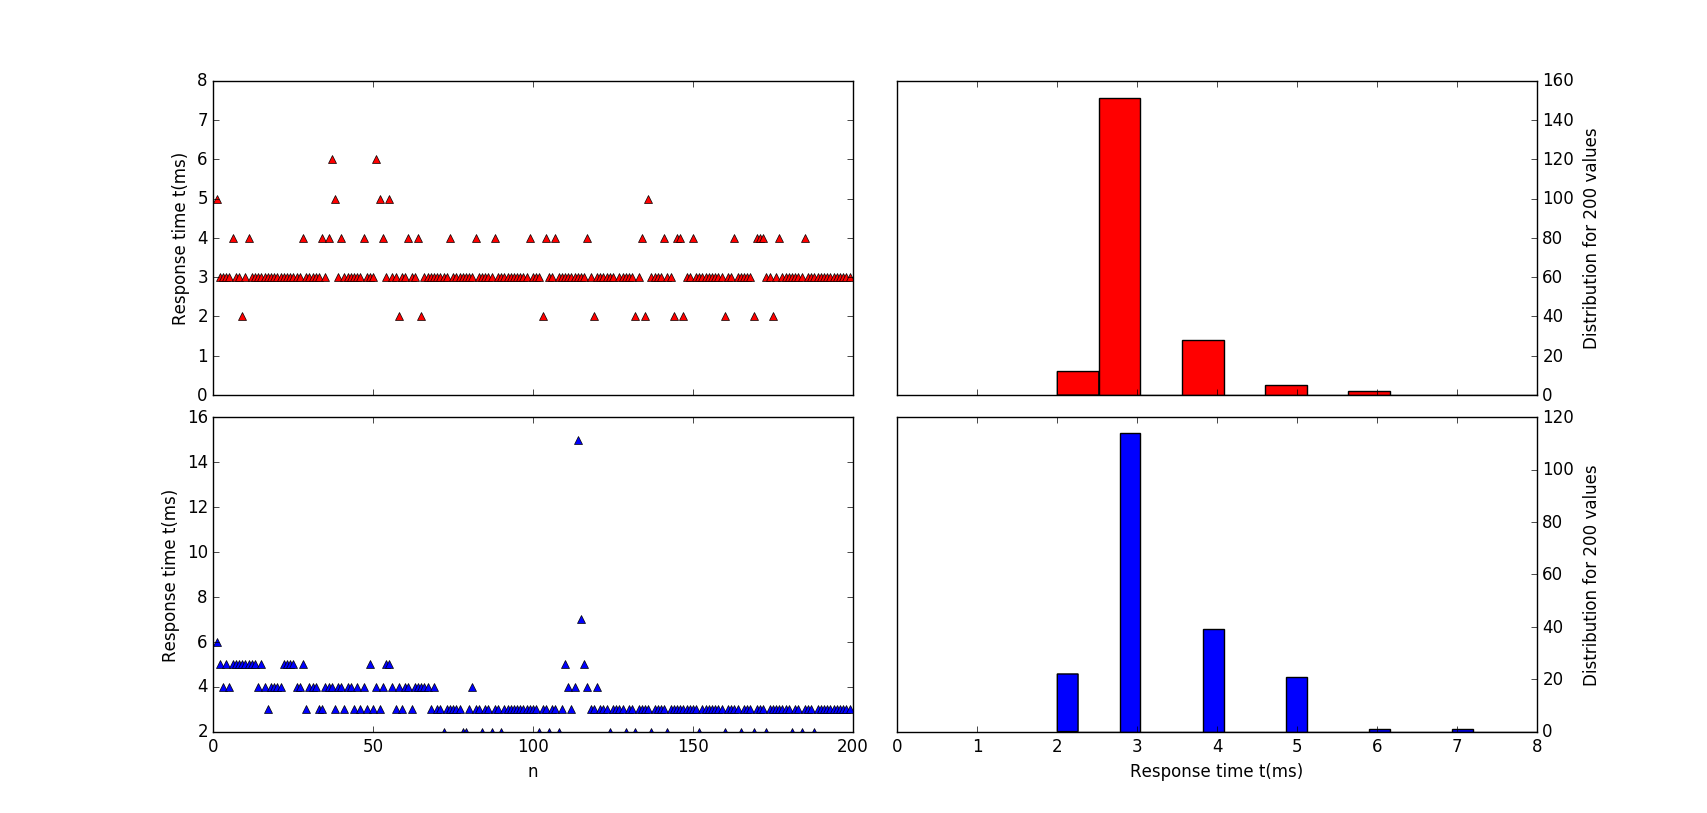
\includegraphics[ width=\linewidth]{plot_time_complexity}
\caption{Response time depending on the exponent n. The top figures corresponds to $A_n$, the bottom ones to $B_n$. Clock routine only returns a response time up to 1ms and mean value is at 3ms.}
\end{figure}

\begin{figure}[H]
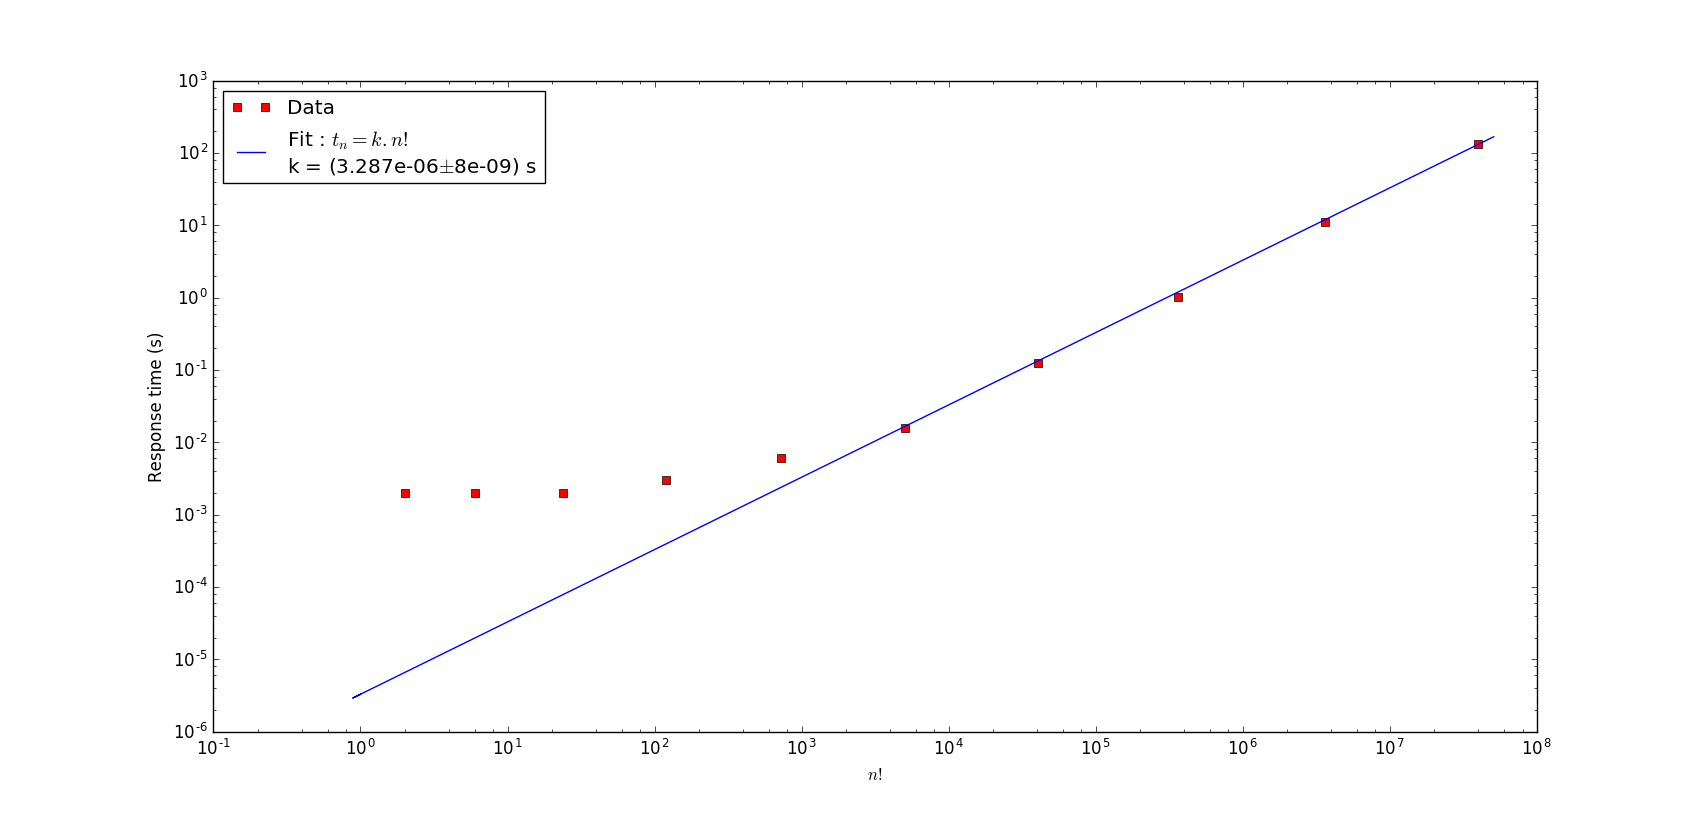
\includegraphics[width=\linewidth]{plot_time_size_matrix}
\caption{Response time with respect to the size of the matrix. Log-log scale was used in order to clearly see both start and end points. The response time of the four first points is about 2ms, which means a relative uncertainty of 50\% and are therefore ignored. A strong correlation between reponse time and the factorial of the size of the matrix can be seen.}
\end{figure}
\newpage
\begin{multicols}{2}


\subsection{SVD decomposition}
SVD method rewrites the matrix A in terms of three matrices U V and S such that
\begin{equation}
A = USV^{T}
\end{equation}

Where U and V are orthonormal matrices respectively formed by the eigenvectors of $A^{T}A$ and $AA^{T}$, and where $S = diag(\sigma_i)$ is a diagonal matrix filled with the singular values (i.e. the square roots of the eigenvalues) of A.\\
The solution to the system of equations $A \bf x \rm = \bf c$ is given by
\begin{equation}
\bf x \rm = A^{\dagger} \bf c
\end{equation}
With $A^{\dagger} = V S^{\dagger} U^{T}$ the pseudo-inverse matrix where $S^{\dagger} = diag(1/\sigma_{i})$.

\subsection{Analysis of the performance of the algorithms}
The performances of both LU and SVD algorithms from the GSL library are examined in this section and are compared to the classical technique using the inversion algorithm from section 1.
Time response is measured for matrices with increasing size and behaviour when approaching a singular matrix
\footnote{A matrix is said to be singular when at least one of its rows or columns is linearly dependent of the others. Since coefficients are floating numbers it seems unlikely that one will get a singular matrix, but they can approach a set of values such that in the limit the matrix would be.}
 is analyzed.
\end{multicols}

\begin{figure}[H]
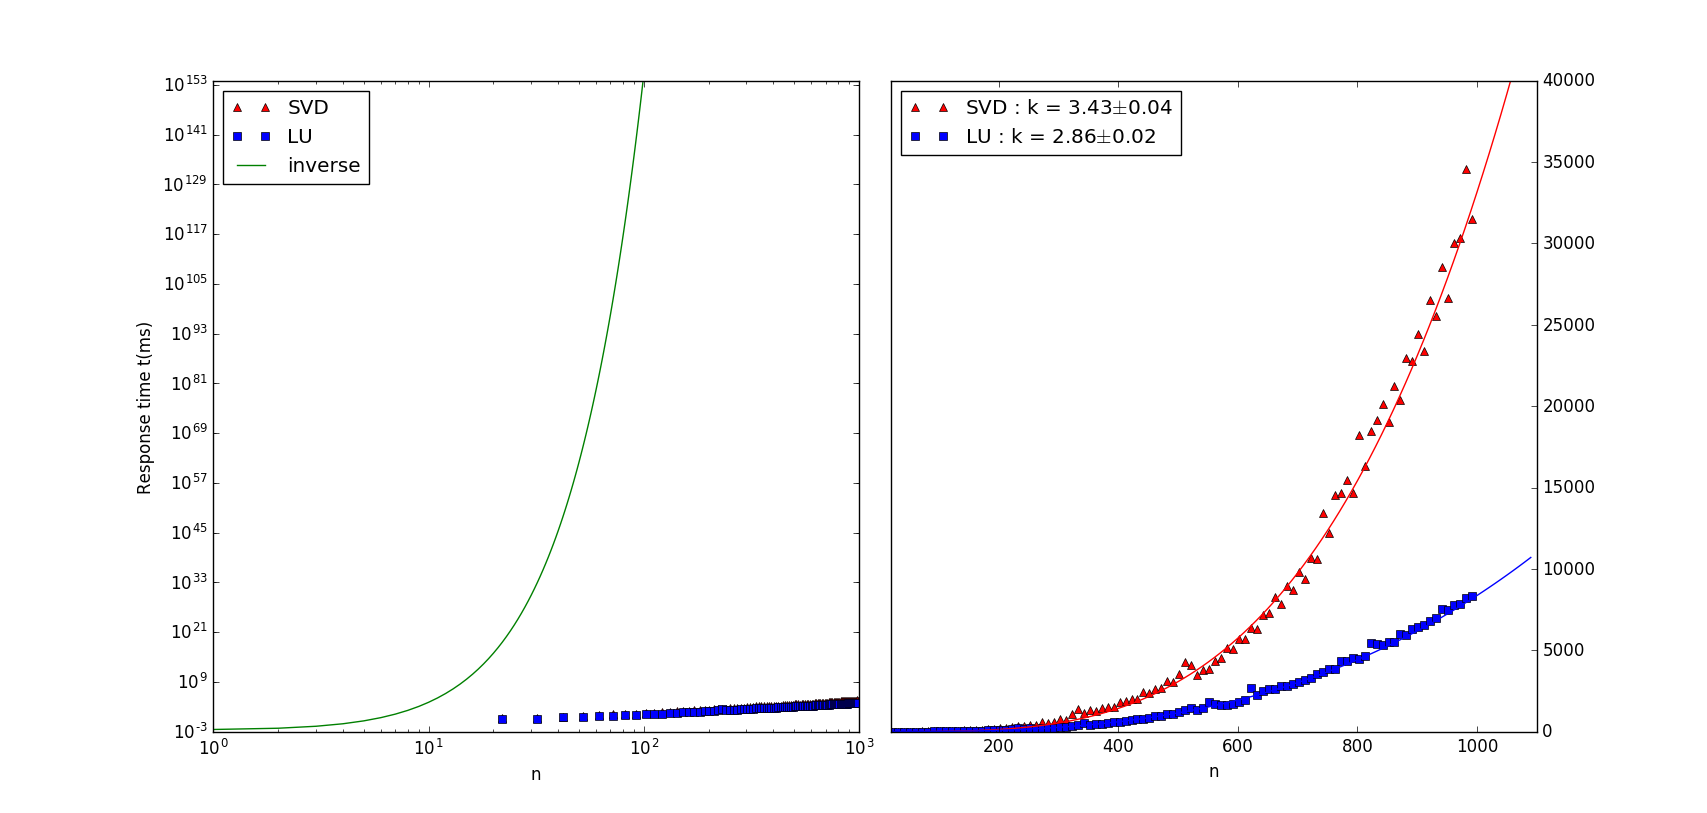
\includegraphics[width = \linewidth]{SVD_LU_inverse}
\caption{Response time relative to the dimension of the matrix. The left graph is log-log and the inverse is plotted using (7) and the coefficient in Fig. 2. The right graph is linear in both axes. Fitting via least squares allow us to determine the exponents k.}
\end{figure}

\begin{multicols}{2}

\subsubsection{Response time}
Both SVD and LU techniques are more efficients than the inverse method and follow a power law in n. Least square fitting gives us the following relations
\begin{equation}
t_{\text{\tiny SVD}} \propto n^{3.43 \pm 0.04}  \    \ t_{\text{\tiny LU}} \propto n^{2.86 \pm 0.02}
\end{equation}

LU technique seems therefore to be more efficient than SVD method.


\subsubsection{Behaviour of the solution when approaching a singular matrix}
A singular matrix can be approached by writing one of its rows as a linear combination of the others. However, one of the coefficients is slighy changed around its singular value

\begin{equation}
\begin{pmatrix}
a & b & c \\
d & e & f\\
a & b & c\\
\end{pmatrix}
\longrightarrow
\begin{pmatrix}
a & b & c \\
d & e & f\\
a & b & c+\epsilon \\
\end{pmatrix}
, |\epsilon | > 0
\end{equation}

The behaviour was studied for the following $3 \times 3$ matrix

\begin{equation}
\begin{pmatrix}
1 & 1 & 1\\
1 & 2 & -1\\
2 & 3 & \varepsilon
\end{pmatrix}
\end{equation}

Where $\epsilon$ varies from -0.1 to 0.1. One can check that if $\epsilon = 0$ the matrix becomes singular. 

\end{multicols}

\begin{figure}[H]
\vspace{-40pt}
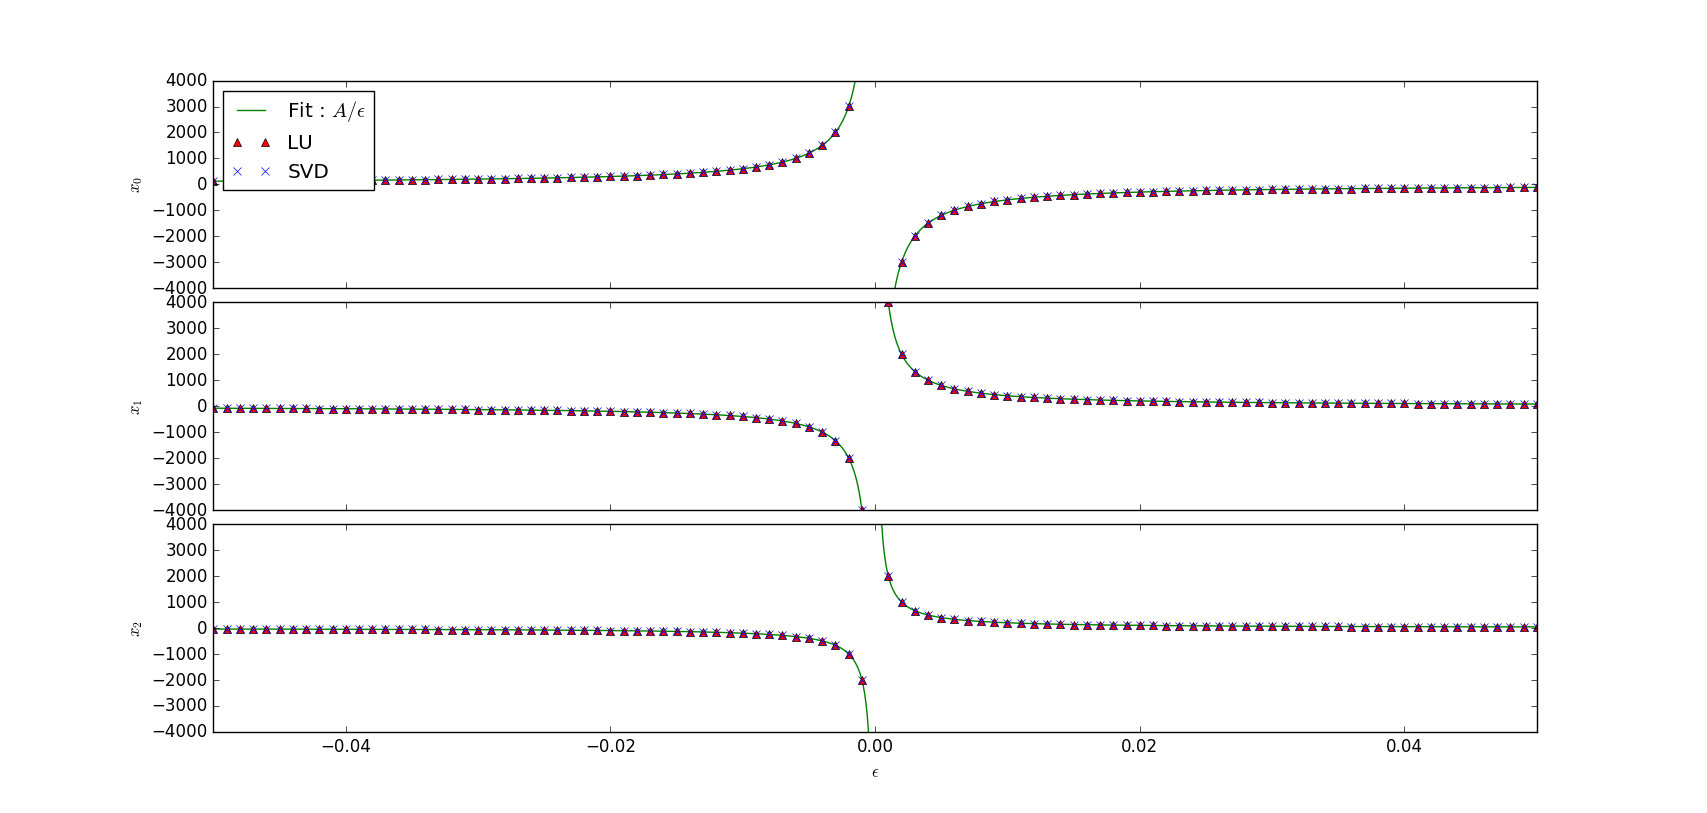
\includegraphics[width = \linewidth]{approaching_singular}
\caption{Change of the components of the solution of the linear system when approaching a singular matrix. In this case the matrix is singular for $\epsilon = 0$ and we see all the components diverge around this value.}
\end{figure}

\begin{multicols}{2}
As shown in Fig. 4 the three components of the solution vector diverge around 0 for both LU and SVD. They both diverge following an inverse law, hence
\begin{equation}
x_{\epsilon} \propto \frac{1}{\epsilon}
\end{equation}

It should be noted that LU methods return NaN when computing the solution for $\epsilon = 0$. On the other hand, SVD returns a really high value.\\

\subsubsection{Conclusion on performances}

LU method appears to be the best candidate when dealing with linear systems. SVD method might be used for matrices with dimension of 700 or less. However for larger matrices, LU should be prefered since it becomes a lot quicker than SVD.\\
If one does not know whether the matrix might be singular or not, LU method should be used in order to avoid any issues.

\section{Physics Problem : cable-controlled camera}

\subsection{Parametrization}
We study in this section the tension in the three cables of a cable-controlled camera used for instance in stadiums. The camera is approximated by a point where all the mass $M = 40 kg$ is concentrated and the three cables are all connected to both the camera and drums fixed on the roof.
By changing the length of the cable, the camera is moved in the 3D space spanned by the 3 cables. In this case we consider that the camera is at a fixed height such that $H_{camera} = 0 m$ and $H_{roof} = 10 m$ and we decide to restrict the study of the tension in the horizontal plane of the camera. The three attachment points form an equilateral triangle where the distance from them to the center is $b = 80 m$ (see Figure 6a). Simple trigonometric relations allow us to find that the field has a the dimensions $L_x = \frac{3}{2}b$ and $L_y = \sqrt{3}b$.\\
From statics we know that we need the sum of all the forces to vanish (moments or torques will not be needed here). Therefore the problem can be expressed in its most general form as

\begin{equation}
\begin{cases}
T_{1x} + T_{2x} + T_{3x} = 0\\
T_{1y} + T_{2y} + T_{3y} = 0\\
T_{1z} + T_{2z} + T_{3z} = mg
\end{cases}
\end{equation}

However we do not need to solve directly this system. We know that the modulus of a vector can be linked in spherical coordinates to two angles $\theta$ and $\phi$. Hence, since we know the position of the point where we want to solve this system we can for each pair $(x,y)$ define three vectors $\bf MM_1$, $\bf MM2$, $\bf MM_3$ (see FIgure 5) that we can rewrite in spherical coordinates as

\begin{equation}
\frac{\bf MM_i}{|\bf MM_i \rm |} \rm = \cos \theta_i \cos\phi_i \bf \hat i \rm + \cos \theta_i \sin\phi_i \bf \hat j \rm +  \sin \theta_i \bf \hat k
\end{equation}

$\theta_i = acos \frac{z_i - z}{\sqrt{(x_i - x)^2 + (y_i - y)^2 + (z_i - z)^2}}$, $\phi_i = atan \frac{y_i - y}{x_i - x}$\\

Because cables can only pull, the tension vectors $\bf T_i$ will always point in the direction of $\bf MM_i$. Hence the following relation holds
\begin{equation}
\bf T_i \rm = |\bf T_i \rm | \frac{\bf MM_i}{|\bf MM_i\rm |}
\end{equation}

\end{multicols}

\begin{figure}[H]
\centering
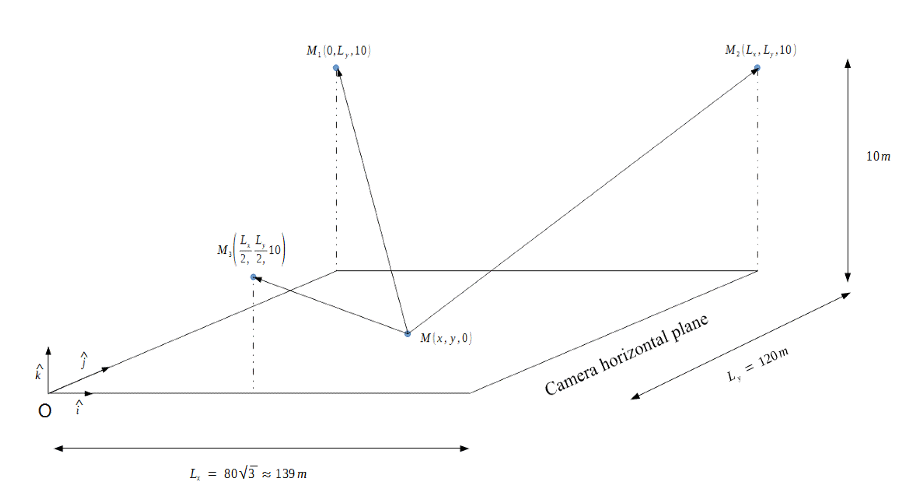
\includegraphics[width = 0.7\linewidth]{sketch}
\caption{Sketch showing the location of the different attachment points and position vectors.}
\end{figure}

\begin{figure}[H]
\centering
\subfloat[Top-view (cables = red, field = blue)]{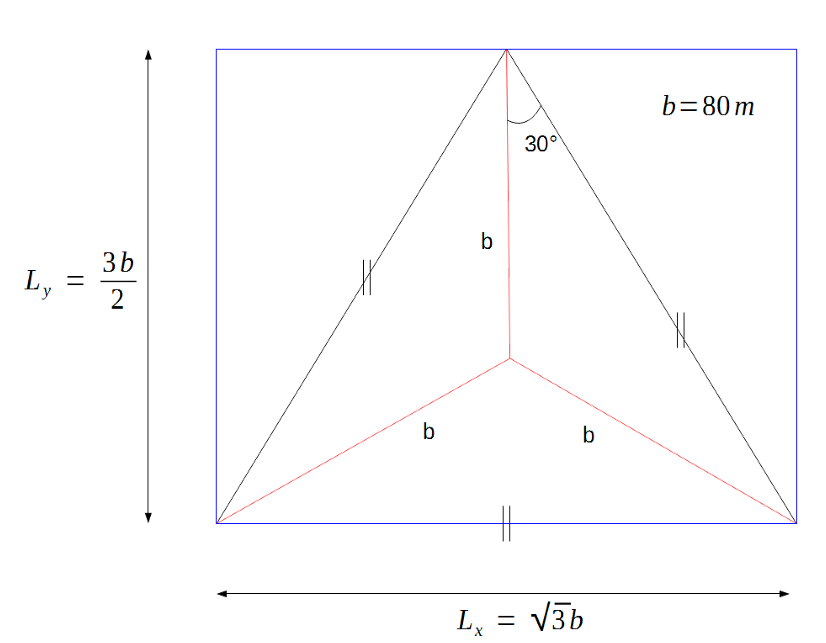
\includegraphics[width =0.49\textwidth]{top_view}}
\subfloat[Parametrization of the vectors]{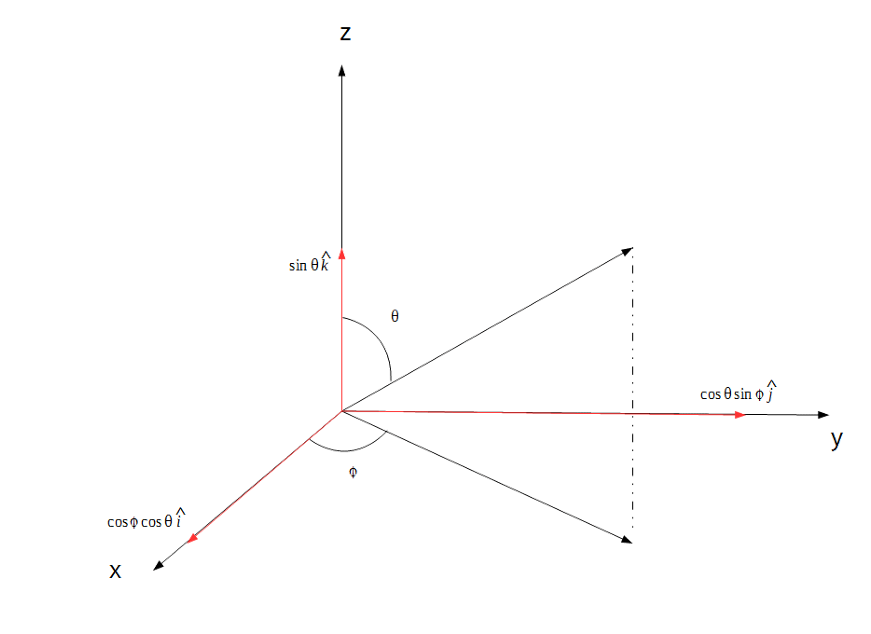
\includegraphics[width =0.49\textwidth]{parametrization}}
\caption{Simple trigonometric relations allow us to find the dimensions of the field. Vectors are defined in spherical coordinates following the convention $0 \leq \theta \leq \pi$, $0 \leq \phi < 2\pi$.}
\end{figure}

\begin{multicols}{2}
Using this parametrization we can rewrite our system in the following matrix form

\begin{gather*}
A \bf T \rm = \bf W \rm\\
\small
\begin{pmatrix}
\cos \theta_1 \cos \phi_1 & cos \theta_2 \cos \phi_2 & \cos \theta_3 \cos\phi_3\\
\cos \theta_1 \sin \phi_1 & cos \theta_2 \sin \phi_2 & \cos \theta_3 \sin \phi_3\\
\sin \theta_1 & \sin \theta_2 & \sin \theta_3
\end{pmatrix}
\begin{pmatrix}
T_1\\
T_2\\
T_3
\end{pmatrix}
=
\begin{pmatrix}
0\\
0\\
mg
\end{pmatrix}
\normalsize
\end{gather*}


Thus, by computing the six angles $\theta$ and $\phi$ for a set of points $(x,y)$ we can use LU method to find the solution of the problem. However since we used spherical coordinates we should expect our solution vector $\bf T$ to contain only positive values. If for instance we consider the case where $\phi_3 \equiv 0\ \ [\pi]$ which corresponds to the x-axis we automatically see from the second equation that we have

\begin{equation}
\frac{T_1}{T_2} = - \frac{\cos \theta_2 \sin \phi2}{\cos \theta_1 \sin \phi_1}
\end{equation} 

Since in this problem all $\theta$ are limited to $[0,\pi/2]$ (0 if the camera is just under the point, $\pi/2$ if the camera stays in the plane but is at infinity) and since $\sin \phi_1 , \sin \phi_2 > 0$ we get $T_1 \propto -T_2$ which should not be allowed.\\
It therefore means the algorithm can actually compute unphysical solutions
\footnote{Another way to look at it is to consider the case where one of the cables is removed (tension of 0). The system will find an equilibrium along the line formed by the two attachment points. If now we put our cable back and apply a force the system will only be moved in the direction of the third attachment point since cables can only pull. By making the same reasoning for the three cables we see that the spanned area will correspond to a triangle which implies positions outside of this triangle cannot be reached.}
 and in order to avoid them, we restrict our data to positive vectors $\bf T$ only.
\end{multicols}

\begin{figure}[H]
\includegraphics[width = \linewidth]{Tension_cables}
\caption{Tension in the cables in the camera hozritontal plane with a resolution of 50cm x 50cm. White zones correspond to places where there is no physical solution in this configuration.}
\end{figure}

\begin{multicols}{2}
\subsection{Analysis of the solution}

As expected the only allowed solutions fit inside the triangle spanned by the three attachment points. Each pair of graphs is axially symmetric under the altitude of the side of the triangle formed by the two attachment points (see Figure 6a). For instance $T_1$ is the symmetric of $T_2$ with the altitude of the side $M_1 M_2$ as axis of symmetry. This makes sense given the symmetry of the problem (equilateral triangle).\\
If we look at $T_1$, we see its lowest value is reached along the line $M_3 M_2$ which is logical given that this configuration is equivalent to a two-cables system. $T_1$ also reach its lowest value when approaching $ M_1$. This is a bit more supprising since one could think that in order to pull the camera towards its attachment point the cable would need to increase the force it is applying. One explanation would be that the x and y components of the cables 2 and 3 cancel each other out and only the vertical component of $T_1$ is non-trivial.\\
The highest value on the other hand is reached when approaching the two other points $M_2$ and $M_3$ (see Figure 7). This once again makes sense since this area corresponds to the place where the tension in one of the other cables is the lowest and therefore in order to compenstate the other cable force the tension in cable 1 needs to increase. This is better shown in Figure 8 where we can see that the overall tension (the sum) is smooth everywhere except at the attachment points.\\
The maximum tension is about 40,000 N which is equivalent to a cable weighting 4 tons. This seems a bit high but it could be explained by the fact that tensions do not only cancel each other out in the z direction but in all of 
 

\begin{figure}[H]
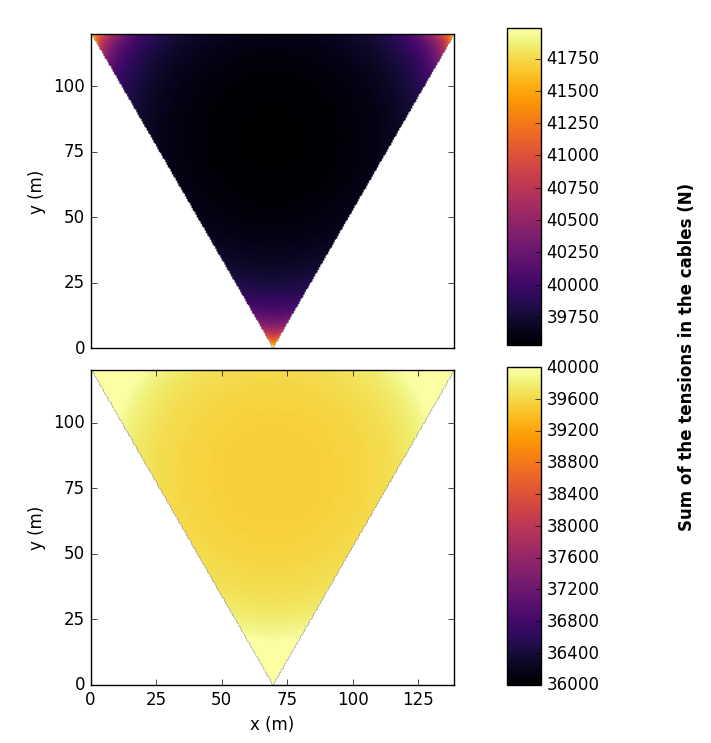
\includegraphics[width = \linewidth]{sum_tension}
\caption{Sum of all the tensions in the cables. The bottom figure has its maximum value at 40,000 N in order to show the smoothness of the values. As shown in the top figure the overall tension rises when approaching the attachment point.} 
\end{figure}

them. This implies that each cable apply a force on the others which therefore increase the overall tension.

\end{multicols}

\begin{thebibliography}{1}
\bibitem{ref}
Valérie Perrier, Roger Mohr.
\textit{La Decomposition en Valeurs Singulieres Analyse numerique et Application a la Vision}.
Ensimag et Laboratoire Jean Kuntzmann,
\\\texttt{http://ensimag.grenoble-inp.fr/servlet/com.univ.collaboratif.utils.LectureFichiergw?ID\_FICHIER=1309510\\187923\&ID\_FICHE=247941\&INLINE=FALSE}
\end{thebibliography}

\end{document}